% Options for packages loaded elsewhere
\PassOptionsToPackage{unicode}{hyperref}
\PassOptionsToPackage{hyphens}{url}
\PassOptionsToPackage{dvipsnames,svgnames,x11names}{xcolor}
%
\documentclass[
  10pt,
  dvipsnames, enabledeprecatedfontcommands]{scrartcl}
\title{Bayesian analysis of the NESTA study of interventions against
verbal aggression online \linebreak  Technical Report}
\author{Rafal Urbaniak}
\date{}

\usepackage{amsmath,amssymb}
\usepackage{lmodern}
\usepackage{iftex}
\ifPDFTeX
  \usepackage[T1]{fontenc}
  \usepackage[utf8]{inputenc}
  \usepackage{textcomp} % provide euro and other symbols
\else % if luatex or xetex
  \usepackage{unicode-math}
  \defaultfontfeatures{Scale=MatchLowercase}
  \defaultfontfeatures[\rmfamily]{Ligatures=TeX,Scale=1}
\fi
% Use upquote if available, for straight quotes in verbatim environments
\IfFileExists{upquote.sty}{\usepackage{upquote}}{}
\IfFileExists{microtype.sty}{% use microtype if available
  \usepackage[]{microtype}
  \UseMicrotypeSet[protrusion]{basicmath} % disable protrusion for tt fonts
}{}
\makeatletter
\@ifundefined{KOMAClassName}{% if non-KOMA class
  \IfFileExists{parskip.sty}{%
    \usepackage{parskip}
  }{% else
    \setlength{\parindent}{0pt}
    \setlength{\parskip}{6pt plus 2pt minus 1pt}}
}{% if KOMA class
  \KOMAoptions{parskip=half}}
\makeatother
\usepackage{xcolor}
\IfFileExists{xurl.sty}{\usepackage{xurl}}{} % add URL line breaks if available
\IfFileExists{bookmark.sty}{\usepackage{bookmark}}{\usepackage{hyperref}}
\hypersetup{
  pdftitle={Bayesian analysis of the NESTA study of interventions against verbal aggression online Technical Report},
  pdfauthor={Rafal Urbaniak},
  colorlinks=true,
  linkcolor={Maroon},
  filecolor={Maroon},
  citecolor={Blue},
  urlcolor={blue},
  pdfcreator={LaTeX via pandoc}}
\urlstyle{same} % disable monospaced font for URLs
\usepackage{color}
\usepackage{fancyvrb}
\newcommand{\VerbBar}{|}
\newcommand{\VERB}{\Verb[commandchars=\\\{\}]}
\DefineVerbatimEnvironment{Highlighting}{Verbatim}{commandchars=\\\{\}}
% Add ',fontsize=\small' for more characters per line
\usepackage{framed}
\definecolor{shadecolor}{RGB}{248,248,248}
\newenvironment{Shaded}{\begin{snugshade}}{\end{snugshade}}
\newcommand{\AlertTok}[1]{\textcolor[rgb]{0.94,0.16,0.16}{#1}}
\newcommand{\AnnotationTok}[1]{\textcolor[rgb]{0.56,0.35,0.01}{\textbf{\textit{#1}}}}
\newcommand{\AttributeTok}[1]{\textcolor[rgb]{0.77,0.63,0.00}{#1}}
\newcommand{\BaseNTok}[1]{\textcolor[rgb]{0.00,0.00,0.81}{#1}}
\newcommand{\BuiltInTok}[1]{#1}
\newcommand{\CharTok}[1]{\textcolor[rgb]{0.31,0.60,0.02}{#1}}
\newcommand{\CommentTok}[1]{\textcolor[rgb]{0.56,0.35,0.01}{\textit{#1}}}
\newcommand{\CommentVarTok}[1]{\textcolor[rgb]{0.56,0.35,0.01}{\textbf{\textit{#1}}}}
\newcommand{\ConstantTok}[1]{\textcolor[rgb]{0.00,0.00,0.00}{#1}}
\newcommand{\ControlFlowTok}[1]{\textcolor[rgb]{0.13,0.29,0.53}{\textbf{#1}}}
\newcommand{\DataTypeTok}[1]{\textcolor[rgb]{0.13,0.29,0.53}{#1}}
\newcommand{\DecValTok}[1]{\textcolor[rgb]{0.00,0.00,0.81}{#1}}
\newcommand{\DocumentationTok}[1]{\textcolor[rgb]{0.56,0.35,0.01}{\textbf{\textit{#1}}}}
\newcommand{\ErrorTok}[1]{\textcolor[rgb]{0.64,0.00,0.00}{\textbf{#1}}}
\newcommand{\ExtensionTok}[1]{#1}
\newcommand{\FloatTok}[1]{\textcolor[rgb]{0.00,0.00,0.81}{#1}}
\newcommand{\FunctionTok}[1]{\textcolor[rgb]{0.00,0.00,0.00}{#1}}
\newcommand{\ImportTok}[1]{#1}
\newcommand{\InformationTok}[1]{\textcolor[rgb]{0.56,0.35,0.01}{\textbf{\textit{#1}}}}
\newcommand{\KeywordTok}[1]{\textcolor[rgb]{0.13,0.29,0.53}{\textbf{#1}}}
\newcommand{\NormalTok}[1]{#1}
\newcommand{\OperatorTok}[1]{\textcolor[rgb]{0.81,0.36,0.00}{\textbf{#1}}}
\newcommand{\OtherTok}[1]{\textcolor[rgb]{0.56,0.35,0.01}{#1}}
\newcommand{\PreprocessorTok}[1]{\textcolor[rgb]{0.56,0.35,0.01}{\textit{#1}}}
\newcommand{\RegionMarkerTok}[1]{#1}
\newcommand{\SpecialCharTok}[1]{\textcolor[rgb]{0.00,0.00,0.00}{#1}}
\newcommand{\SpecialStringTok}[1]{\textcolor[rgb]{0.31,0.60,0.02}{#1}}
\newcommand{\StringTok}[1]{\textcolor[rgb]{0.31,0.60,0.02}{#1}}
\newcommand{\VariableTok}[1]{\textcolor[rgb]{0.00,0.00,0.00}{#1}}
\newcommand{\VerbatimStringTok}[1]{\textcolor[rgb]{0.31,0.60,0.02}{#1}}
\newcommand{\WarningTok}[1]{\textcolor[rgb]{0.56,0.35,0.01}{\textbf{\textit{#1}}}}
\usepackage{graphicx}
\makeatletter
\def\maxwidth{\ifdim\Gin@nat@width>\linewidth\linewidth\else\Gin@nat@width\fi}
\def\maxheight{\ifdim\Gin@nat@height>\textheight\textheight\else\Gin@nat@height\fi}
\makeatother
% Scale images if necessary, so that they will not overflow the page
% margins by default, and it is still possible to overwrite the defaults
% using explicit options in \includegraphics[width, height, ...]{}
\setkeys{Gin}{width=\maxwidth,height=\maxheight,keepaspectratio}
% Set default figure placement to htbp
\makeatletter
\def\fps@figure{htbp}
\makeatother
\setlength{\emergencystretch}{3em} % prevent overfull lines
\providecommand{\tightlist}{%
  \setlength{\itemsep}{0pt}\setlength{\parskip}{0pt}}
\setcounter{secnumdepth}{-\maxdimen} % remove section numbering
\usepackage{booktabs}
\usepackage{longtable}
\usepackage{array}
\usepackage{multirow}
\usepackage{wrapfig}
\usepackage{float}
\usepackage{colortbl}
\usepackage{pdflscape}
\usepackage{tabu}
\usepackage{threeparttable}
\usepackage{threeparttablex}
\usepackage[normalem]{ulem}
\usepackage{makecell}
\usepackage{xcolor}
\ifLuaTeX
  \usepackage{selnolig}  % disable illegal ligatures
\fi

\begin{document}
\maketitle

\tableofcontents

\hypertarget{data-and-exploration}{%
\section{Data and exploration}\label{data-and-exploration}}

\vspace{1mm}
\scriptsize

\begin{Shaded}
\begin{Highlighting}[]
\NormalTok{Hate }\OtherTok{\textless{}{-}} \FunctionTok{readRDS}\NormalTok{(}\AttributeTok{file =} \StringTok{"datasets/RAWNESTA/Hate.rds"}\NormalTok{)}
\NormalTok{Comments }\OtherTok{\textless{}{-}} \FunctionTok{readRDS}\NormalTok{(}\AttributeTok{file =} \StringTok{"datasets/RAWNESTA/Comments.rds"}\NormalTok{)}
\NormalTok{summaries }\OtherTok{\textless{}{-}} \FunctionTok{read.csv}\NormalTok{(}\AttributeTok{file =} \StringTok{"datasets/Summaries.csv"}\NormalTok{)}

\NormalTok{dates }\OtherTok{\textless{}{-}} \FunctionTok{colnames}\NormalTok{(Hate)[}\SpecialCharTok{{-}}\DecValTok{1}\NormalTok{]}
\NormalTok{dates }\OtherTok{\textless{}{-}} \FunctionTok{as.Date}\NormalTok{(dates)}
\NormalTok{startDate }\OtherTok{\textless{}{-}}\NormalTok{ dates[}\DecValTok{1}\NormalTok{]}
\NormalTok{interventionDate }\OtherTok{\textless{}{-}} \StringTok{"2020{-}07{-}08"}
\NormalTok{observationDate }\OtherTok{\textless{}{-}} \StringTok{"2020{-}09{-}09"}
\NormalTok{end }\OtherTok{\textless{}{-}}\NormalTok{ dates[}\FunctionTok{length}\NormalTok{(dates)]}

\NormalTok{periods }\OtherTok{\textless{}{-}} \FunctionTok{numeric}\NormalTok{(}\FunctionTok{length}\NormalTok{(dates))}
\NormalTok{periods }\OtherTok{\textless{}{-}} \FunctionTok{ifelse}\NormalTok{(dates }\SpecialCharTok{\textless{}}\NormalTok{ interventionDate, }\StringTok{"pre{-}treatment"}\NormalTok{, periods)}
\NormalTok{periods }\OtherTok{\textless{}{-}} \FunctionTok{ifelse}\NormalTok{(dates }\SpecialCharTok{\textgreater{}=}\NormalTok{ interventionDate }\SpecialCharTok{\&}\NormalTok{ dates }\SpecialCharTok{\textless{}}\NormalTok{ observationDate,}
    \StringTok{"treatment"}\NormalTok{, periods)}
\NormalTok{periods }\OtherTok{\textless{}{-}} \FunctionTok{ifelse}\NormalTok{(dates }\SpecialCharTok{\textgreater{}=}\NormalTok{ observationDate, }\StringTok{"post{-}treatment"}\NormalTok{, periods)}

\NormalTok{hateTS }\OtherTok{\textless{}{-}} \FunctionTok{as.data.frame}\NormalTok{(}\FunctionTok{colSums}\NormalTok{(Hate[, }\SpecialCharTok{{-}}\DecValTok{1}\NormalTok{]))}
\NormalTok{hateTS}\SpecialCharTok{$}\NormalTok{date }\OtherTok{\textless{}{-}} \FunctionTok{as.Date}\NormalTok{(}\FunctionTok{rownames}\NormalTok{(hateTS))}
\FunctionTok{rownames}\NormalTok{(hateTS) }\OtherTok{\textless{}{-}} \ConstantTok{NULL}
\FunctionTok{colnames}\NormalTok{(hateTS) }\OtherTok{\textless{}{-}} \FunctionTok{c}\NormalTok{(}\StringTok{"attacks"}\NormalTok{, }\StringTok{"date"}\NormalTok{)}
\NormalTok{hateTS}\SpecialCharTok{$}\NormalTok{periods }\OtherTok{\textless{}{-}}\NormalTok{ periods}

\NormalTok{interventions }\OtherTok{\textless{}{-}} \FunctionTok{readRDS}\NormalTok{(}\AttributeTok{file =} \StringTok{"datasets/interventions.rds"}\NormalTok{)}
\NormalTok{interventionsTS }\OtherTok{\textless{}{-}} \FunctionTok{as.data.frame}\NormalTok{(}\FunctionTok{table}\NormalTok{(interventions}\SpecialCharTok{$}\NormalTok{day))}
\NormalTok{interventionsTS}\SpecialCharTok{$}\NormalTok{Var1 }\OtherTok{\textless{}{-}} \FunctionTok{as.Date}\NormalTok{(interventionsTS}\SpecialCharTok{$}\NormalTok{Var1)}
\FunctionTok{colnames}\NormalTok{(interventionsTS) }\OtherTok{\textless{}{-}} \FunctionTok{c}\NormalTok{(}\StringTok{"date"}\NormalTok{, }\StringTok{"interventions"}\NormalTok{)}

\NormalTok{periodsDF }\OtherTok{\textless{}{-}} \FunctionTok{merge}\NormalTok{(}\AttributeTok{x =}\NormalTok{ hateTS, }\AttributeTok{y =}\NormalTok{ interventionsTS, }\AttributeTok{by =} \StringTok{"date"}\NormalTok{, }\AttributeTok{all.x =} \ConstantTok{TRUE}\NormalTok{)}

\NormalTok{idx }\OtherTok{\textless{}{-}} \FunctionTok{c}\NormalTok{(}\DecValTok{1}\NormalTok{, }\FunctionTok{diff}\NormalTok{(periodsDF}\SpecialCharTok{$}\NormalTok{date))}
\NormalTok{i2 }\OtherTok{\textless{}{-}} \FunctionTok{c}\NormalTok{(}\DecValTok{1}\NormalTok{, }\FunctionTok{which}\NormalTok{(idx }\SpecialCharTok{!=} \DecValTok{1}\NormalTok{), }\FunctionTok{nrow}\NormalTok{(periodsDF) }\SpecialCharTok{+} \DecValTok{1}\NormalTok{)}
\NormalTok{periodsDF}\SpecialCharTok{$}\NormalTok{grp }\OtherTok{\textless{}{-}} \FunctionTok{rep}\NormalTok{(}\DecValTok{1}\SpecialCharTok{:}\FunctionTok{length}\NormalTok{(}\FunctionTok{diff}\NormalTok{(i2)), }\FunctionTok{diff}\NormalTok{(i2))}

\NormalTok{periodsDF}\SpecialCharTok{$}\NormalTok{interventions[}\FunctionTok{is.na}\NormalTok{(periodsDF}\SpecialCharTok{$}\NormalTok{interventions) }\SpecialCharTok{\&}\NormalTok{ periodsDF}\SpecialCharTok{$}\NormalTok{periods }\SpecialCharTok{==}
    \StringTok{"treatment"}\NormalTok{] }\OtherTok{\textless{}{-}} \DecValTok{0}

\NormalTok{periodsPlot }\OtherTok{\textless{}{-}} \FunctionTok{ggplot}\NormalTok{(periodsDF) }\SpecialCharTok{+} \FunctionTok{geom\_line}\NormalTok{(}\FunctionTok{aes}\NormalTok{(}\AttributeTok{x =}\NormalTok{ date, }\AttributeTok{y =}\NormalTok{ attacks,}
    \AttributeTok{group =}\NormalTok{ grp), }\AttributeTok{alpha =} \FloatTok{0.8}\NormalTok{, }\AttributeTok{size =} \FloatTok{0.6}\NormalTok{) }\SpecialCharTok{+} \FunctionTok{geom\_line}\NormalTok{(}\FunctionTok{aes}\NormalTok{(}\AttributeTok{x =}\NormalTok{ date, }\AttributeTok{y =}\NormalTok{ interventions,}
    \AttributeTok{group =}\NormalTok{ grp), }\AttributeTok{alpha =} \FloatTok{0.8}\NormalTok{, }\AttributeTok{size =} \FloatTok{0.6}\NormalTok{) }\SpecialCharTok{+} \FunctionTok{geom\_vline}\NormalTok{(}\AttributeTok{xintercept =}\NormalTok{ startDate,}
    \AttributeTok{lty =} \DecValTok{2}\NormalTok{, }\AttributeTok{size =} \FloatTok{0.2}\NormalTok{, }\AttributeTok{alpha =} \FloatTok{0.5}\NormalTok{) }\SpecialCharTok{+} \FunctionTok{geom\_vline}\NormalTok{(}\AttributeTok{xintercept =} \FunctionTok{as.Date}\NormalTok{(interventionDate),}
    \AttributeTok{lty =} \DecValTok{2}\NormalTok{, }\AttributeTok{size =} \FloatTok{0.2}\NormalTok{, }\AttributeTok{alpha =} \FloatTok{0.5}\NormalTok{) }\SpecialCharTok{+} \FunctionTok{geom\_vline}\NormalTok{(}\AttributeTok{xintercept =} \FunctionTok{as.Date}\NormalTok{(observationDate),}
    \AttributeTok{lty =} \DecValTok{2}\NormalTok{, }\AttributeTok{size =} \FloatTok{0.2}\NormalTok{, }\AttributeTok{alpha =} \FloatTok{0.5}\NormalTok{) }\SpecialCharTok{+} \FunctionTok{geom\_vline}\NormalTok{(}\AttributeTok{xintercept =} \FunctionTok{as.Date}\NormalTok{(end),}
    \AttributeTok{lty =} \DecValTok{2}\NormalTok{, }\AttributeTok{size =} \FloatTok{0.2}\NormalTok{, }\AttributeTok{alpha =} \FloatTok{0.5}\NormalTok{) }\SpecialCharTok{+} \FunctionTok{labs}\NormalTok{(}\AttributeTok{title =} \StringTok{"Attacks and interventions time series"}\NormalTok{,}
    \AttributeTok{subtitle =} \StringTok{"no line at data gaps"}\NormalTok{, }\AttributeTok{caption =} \StringTok{"days with data: 81 (pre{-}treatment), 62 (treatment), 72 (post{-}treatment)"}\NormalTok{) }\SpecialCharTok{+}
    \FunctionTok{theme\_tufte}\NormalTok{() }\SpecialCharTok{+} \FunctionTok{theme}\NormalTok{(}\AttributeTok{axis.title.x =} \FunctionTok{element\_blank}\NormalTok{(), }\AttributeTok{plot.caption =} \FunctionTok{element\_text}\NormalTok{(}\AttributeTok{hjust =} \FloatTok{0.5}\NormalTok{,}
    \AttributeTok{face =} \StringTok{"italic"}\NormalTok{)) }\SpecialCharTok{+} \FunctionTok{scale\_x\_date}\NormalTok{(}\AttributeTok{date\_labels =} \StringTok{"\%b \%d"}\NormalTok{, }\AttributeTok{breaks =} \FunctionTok{c}\NormalTok{(startDate,}
    \FunctionTok{as.Date}\NormalTok{(startDate), }\FunctionTok{as.Date}\NormalTok{(interventionDate), }\FunctionTok{as.Date}\NormalTok{(observationDate),}
\NormalTok{    end), }\AttributeTok{limits =} \FunctionTok{c}\NormalTok{(startDate }\SpecialCharTok{{-}} \DecValTok{30}\NormalTok{, end }\SpecialCharTok{+} \DecValTok{10}\NormalTok{)) }\SpecialCharTok{+} \FunctionTok{ylab}\NormalTok{(}\StringTok{"count"}\NormalTok{) }\SpecialCharTok{+} \FunctionTok{annotate}\NormalTok{(}\StringTok{"rect"}\NormalTok{,}
    \AttributeTok{xmin =} \FunctionTok{as.Date}\NormalTok{(interventionDate), }\AttributeTok{xmax =} \FunctionTok{as.Date}\NormalTok{(observationDate),}
    \AttributeTok{ymin =} \SpecialCharTok{{-}}\DecValTok{1}\NormalTok{, }\AttributeTok{ymax =} \DecValTok{360}\NormalTok{, }\AttributeTok{alpha =} \FloatTok{0.2}\NormalTok{, }\AttributeTok{fill =} \StringTok{"darkgreen"}\NormalTok{) }\SpecialCharTok{+} \FunctionTok{ylim}\NormalTok{(}\FunctionTok{c}\NormalTok{(}\SpecialCharTok{{-}}\DecValTok{1}\NormalTok{,}
    \DecValTok{370}\NormalTok{)) }\SpecialCharTok{+} \FunctionTok{annotate}\NormalTok{(}\StringTok{"text"}\NormalTok{, }\AttributeTok{label =} \StringTok{"pre{-}treatment"}\NormalTok{, }\AttributeTok{x =} \FunctionTok{as.Date}\NormalTok{(startDate) }\SpecialCharTok{+}
    \DecValTok{2}\NormalTok{, }\AttributeTok{y =} \DecValTok{370}\NormalTok{, }\AttributeTok{hjust =} \DecValTok{0}\NormalTok{) }\SpecialCharTok{+} \FunctionTok{annotate}\NormalTok{(}\StringTok{"text"}\NormalTok{, }\AttributeTok{label =} \StringTok{"treatment"}\NormalTok{, }\AttributeTok{x =} \FunctionTok{as.Date}\NormalTok{(interventionDate) }\SpecialCharTok{+}
    \DecValTok{2}\NormalTok{, }\AttributeTok{y =} \DecValTok{370}\NormalTok{, }\AttributeTok{hjust =} \DecValTok{0}\NormalTok{) }\SpecialCharTok{+} \FunctionTok{annotate}\NormalTok{(}\StringTok{"text"}\NormalTok{, }\AttributeTok{label =} \StringTok{"post{-}treatment"}\NormalTok{,}
    \AttributeTok{x =} \FunctionTok{as.Date}\NormalTok{(observationDate) }\SpecialCharTok{+} \DecValTok{2}\NormalTok{, }\AttributeTok{y =} \DecValTok{370}\NormalTok{, }\AttributeTok{hjust =} \DecValTok{0}\NormalTok{) }\SpecialCharTok{+} \FunctionTok{annotate}\NormalTok{(}\StringTok{"text"}\NormalTok{,}
    \AttributeTok{label =} \StringTok{"interventions:"}\NormalTok{, }\AttributeTok{x =} \FunctionTok{as.Date}\NormalTok{(interventionDate) }\SpecialCharTok{{-}} \DecValTok{55}\NormalTok{, }\AttributeTok{y =} \DecValTok{15}\NormalTok{,}
    \AttributeTok{hjust =} \DecValTok{0}\NormalTok{) }\SpecialCharTok{+} \FunctionTok{annotate}\NormalTok{(}\StringTok{"text"}\NormalTok{, }\AttributeTok{label =} \StringTok{"attacks:"}\NormalTok{, }\AttributeTok{x =} \FunctionTok{as.Date}\NormalTok{(startDate) }\SpecialCharTok{{-}}
    \DecValTok{30}\NormalTok{, }\AttributeTok{y =} \DecValTok{215}\NormalTok{, }\AttributeTok{hjust =} \DecValTok{0}\NormalTok{)}

\NormalTok{periodsDF}\SpecialCharTok{$}\NormalTok{weekdays }\OtherTok{\textless{}{-}} \FunctionTok{weekdays}\NormalTok{(}\FunctionTok{as.Date}\NormalTok{(periodsDF}\SpecialCharTok{$}\NormalTok{date))}
\NormalTok{periodsDF}\SpecialCharTok{$}\NormalTok{weeks }\OtherTok{\textless{}{-}} \FunctionTok{week}\NormalTok{(}\FunctionTok{as.Date}\NormalTok{(periodsDF}\SpecialCharTok{$}\NormalTok{date))}

\NormalTok{periodsDF}\SpecialCharTok{$}\NormalTok{weekdays }\OtherTok{\textless{}{-}} \FunctionTok{as.factor}\NormalTok{(periodsDF}\SpecialCharTok{$}\NormalTok{weekdays)}
\FunctionTok{levels}\NormalTok{(periodsDF}\SpecialCharTok{$}\NormalTok{weekdays) }\OtherTok{\textless{}{-}} \FunctionTok{c}\NormalTok{(}\StringTok{"Monday"}\NormalTok{, }\StringTok{"Tuesday"}\NormalTok{, }\StringTok{"Wednesday"}\NormalTok{, }\StringTok{"Thursday"}\NormalTok{,}
    \StringTok{"Friday"}\NormalTok{, }\StringTok{"Saturday"}\NormalTok{, }\StringTok{"Sunday"}\NormalTok{)}
\NormalTok{weeksPlot }\OtherTok{\textless{}{-}} \FunctionTok{ggplot}\NormalTok{(periodsDF) }\SpecialCharTok{+} \FunctionTok{geom\_smooth}\NormalTok{(}\FunctionTok{aes}\NormalTok{(}\AttributeTok{x =}\NormalTok{ weekdays, }\AttributeTok{y =}\NormalTok{ attacks,}
    \AttributeTok{group =} \DecValTok{1}\NormalTok{)) }\SpecialCharTok{+} \FunctionTok{geom\_line}\NormalTok{(}\FunctionTok{aes}\NormalTok{(}\AttributeTok{x =}\NormalTok{ weekdays, }\AttributeTok{y =}\NormalTok{ attacks, }\AttributeTok{group =}\NormalTok{ weeks),}
    \AttributeTok{alpha =} \FloatTok{0.1}\NormalTok{) }\SpecialCharTok{+} \FunctionTok{theme\_tufte}\NormalTok{() }\SpecialCharTok{+} \FunctionTok{labs}\NormalTok{(}\AttributeTok{title =} \StringTok{"Personal attacks throught weekdays (six months)"}\NormalTok{,}
    \AttributeTok{subtitle =} \StringTok{"No weekly patterns"}\NormalTok{) }\SpecialCharTok{+} \FunctionTok{xlab}\NormalTok{(}\StringTok{""}\NormalTok{) }\SpecialCharTok{+} \FunctionTok{ylab}\NormalTok{(}\StringTok{"count"}\NormalTok{)}
\end{Highlighting}
\end{Shaded}

\normalsize

For the duration of the project we selected 486 Reddit users and tracked
their activity (with some breaks resulting from API restrictions and
technical issues, which were mostly sorted out in the observation
period), starting on \texttt{r}startDate`, beginning the intervention
period on 2020-07-08, leading to a further observation period starting
on 2020-09-09 and ending on 2020-11-20. The time series of attacks
observed and of interventions conducted can be inspected in Figure
\ref{fig:periodsPlot}.

\begin{figure}[H]

\begin{center}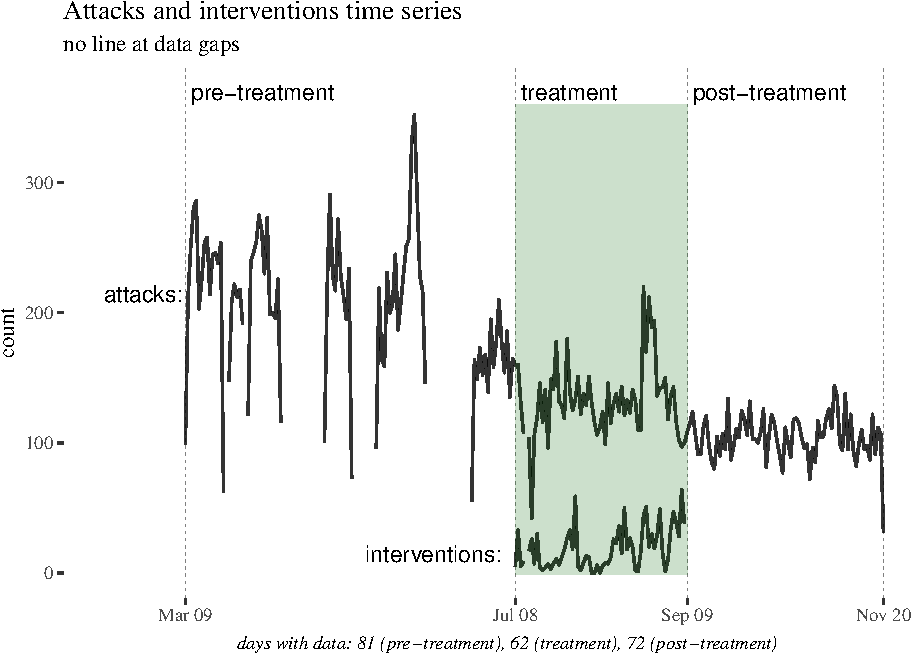
\includegraphics[width=1\linewidth]{technicalReport4_files/figure-latex/periodsPlot-1} \end{center}
\caption{Daily sums of attacks and interventions throughout the three experimental periods, with GAM smoothing (blue).}
\label{fig:periodsPlot}
\end{figure}

Interestingly, no weekly patterns of overall aggressive behavior seem
apparent, as can be seen from plotting multiple weeks alongside, as in
Figure \ref{fig:weeksPlot}.

\begin{figure}[H]

\begin{center}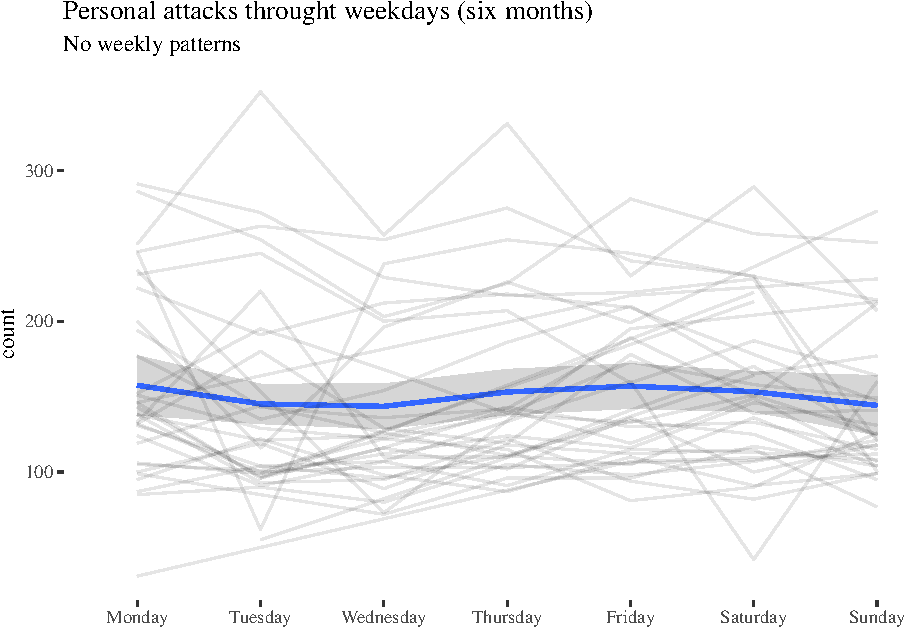
\includegraphics[width=1\linewidth]{technicalReport4_files/figure-latex/weeksPlot-1} \end{center}
\caption{Attack sums from all  weeks in the experimental period plotted against week days. No pattern seems to arise.}
\label{fig:weeksPlot}
\end{figure}

We analyzed the data from two perspective: we ran a before-and after
analysis, comparing the summarized aggression levels before and after
the intervention period (with various additional predictors), and a
time-series perspective, which took a more fine-grained perspective. For
now, we will focus on the Bayesian before-and-after analysis, for which
the data were cleaned and converted into a summarized form, involving
the variables listed in Table \ref{tab:baaVars}.

\vspace{1mm}
\footnotesize

\normalsize

\begin{table}
\centering
\begin{tabular}{ll}
\toprule
variable & explanation\\
\midrule
\cellcolor{gray!6}{AB} & \cellcolor{gray!6}{attacks before (pre-treatment)}\\
AD & attacks during (the treatment period)\\
\cellcolor{gray!6}{AA} & \cellcolor{gray!6}{attacks after (post-treatment)}\\
CB & comments before\\
\cellcolor{gray!6}{CD} & \cellcolor{gray!6}{comments during}\\
CA & comments after\\
\cellcolor{gray!6}{group} & \cellcolor{gray!6}{treatment group}\\
IC & intervention count\\
\bottomrule
\end{tabular}

\caption{Variables involved in the before-and-after analysis.}
\label{tab:baaVars}
\end{table}

Further variables were defined in terms of those, in particular, we will
be predicting \textsf{AdiffS} which is the standardized difference
\textsf{AA}-\textsf{AB}, and \textsf{AdiffS}, which is the standardized
difference \textsf{CA}-\textsf{CB}. The predictors were also
standardized (and named \(\langle\)variable\char`\_name\(\rangle\)S),
and a numerical index for the group (\textsf{groupID}) has been
introduced.

\vspace{1mm}
\footnotesize

\begin{Shaded}
\begin{Highlighting}[]
\NormalTok{summaries}\SpecialCharTok{$}\NormalTok{ABS }\OtherTok{\textless{}{-}} \FunctionTok{standardize}\NormalTok{(summaries}\SpecialCharTok{$}\NormalTok{AB)}
\NormalTok{summaries}\SpecialCharTok{$}\NormalTok{CBS }\OtherTok{\textless{}{-}} \FunctionTok{standardize}\NormalTok{(summaries}\SpecialCharTok{$}\NormalTok{CB)}
\NormalTok{summaries}\SpecialCharTok{$}\NormalTok{AAS }\OtherTok{\textless{}{-}} \FunctionTok{standardize}\NormalTok{(summaries}\SpecialCharTok{$}\NormalTok{AA)}
\NormalTok{summaries}\SpecialCharTok{$}\NormalTok{CAS }\OtherTok{\textless{}{-}} \FunctionTok{standardize}\NormalTok{(summaries}\SpecialCharTok{$}\NormalTok{CA)}
\NormalTok{summaries}\SpecialCharTok{$}\NormalTok{CDS }\OtherTok{\textless{}{-}} \FunctionTok{standardize}\NormalTok{(summaries}\SpecialCharTok{$}\NormalTok{CD)}
\NormalTok{summaries}\SpecialCharTok{$}\NormalTok{ADS }\OtherTok{\textless{}{-}} \FunctionTok{standardize}\NormalTok{(summaries}\SpecialCharTok{$}\NormalTok{AD)}
\NormalTok{summaries}\SpecialCharTok{$}\NormalTok{group }\OtherTok{\textless{}{-}} \FunctionTok{as.factor}\NormalTok{(summaries}\SpecialCharTok{$}\NormalTok{group)}
\NormalTok{summaries}\SpecialCharTok{$}\NormalTok{groupID }\OtherTok{\textless{}{-}} \FunctionTok{as.integer}\NormalTok{(}\FunctionTok{as.factor}\NormalTok{(summaries}\SpecialCharTok{$}\NormalTok{group))}
\end{Highlighting}
\end{Shaded}

\normalsize

The distribution of \textsf{IC} in the treatment groups is visualized in
Figure \ref{fig:interventionsDistro}. Note that the distributions are
somewhat different, even though the total intervention counts are
similar (110 for empathy and 119 for normative). The issue is discussed
in Section XXXXX.

\vspace{1mm}
\footnotesize

\begin{Shaded}
\begin{Highlighting}[]
\NormalTok{interventionsDistro }\OtherTok{\textless{}{-}} \FunctionTok{ggplot}\NormalTok{(summaries[summaries}\SpecialCharTok{$}\NormalTok{group }\SpecialCharTok{!=} \StringTok{"control"}\NormalTok{, ],}
    \FunctionTok{aes}\NormalTok{(}\AttributeTok{x =}\NormalTok{ IC, }\AttributeTok{fill =}\NormalTok{ group)) }\SpecialCharTok{+} \FunctionTok{geom\_bar}\NormalTok{() }\SpecialCharTok{+} \FunctionTok{theme\_tufte}\NormalTok{() }\SpecialCharTok{+} \FunctionTok{xlab}\NormalTok{(}\StringTok{"interventions received"}\NormalTok{) }\SpecialCharTok{+}
    \FunctionTok{labs}\NormalTok{(}\AttributeTok{title =} \StringTok{"Intervention counts in treatment groups"}\NormalTok{) }\SpecialCharTok{+} \FunctionTok{scale\_x\_continuous}\NormalTok{(}\AttributeTok{breaks =} \FunctionTok{seq}\NormalTok{(}\DecValTok{0}\NormalTok{,}
    \DecValTok{40}\NormalTok{, }\DecValTok{5}\NormalTok{))}
\end{Highlighting}
\end{Shaded}

\normalsize

\begin{figure}[H]

\begin{center}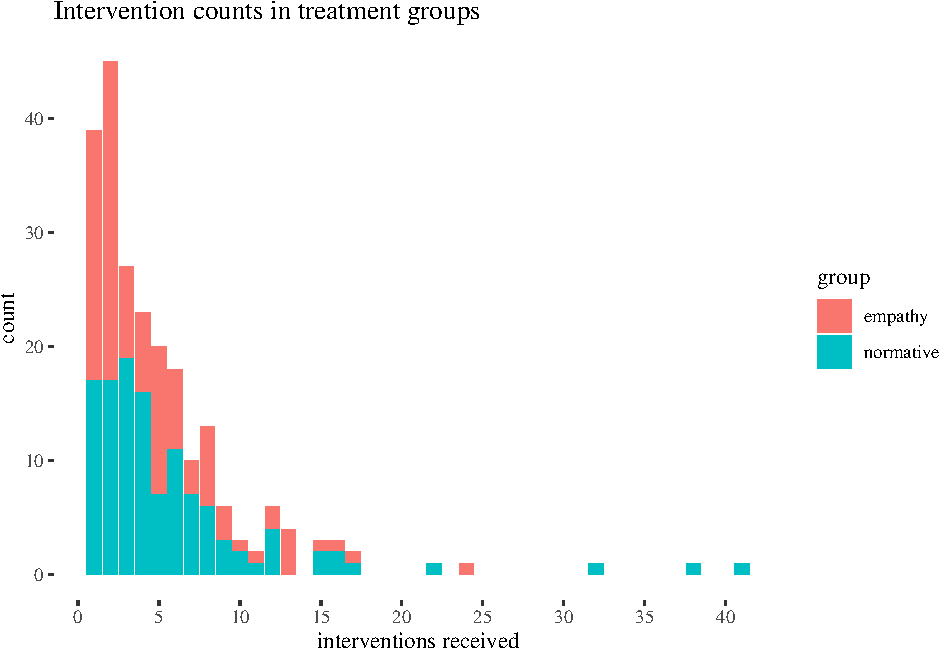
\includegraphics[width=1\linewidth]{technicalReport4_files/figure-latex/interventionsDistro-1} \end{center}
\caption{Distribution of daily interventions, by treatment group.}
\label{fig:interventionsDistro}
\end{figure}

Second, when we look at the distribution of standardized difference in
attacks, when restricted to (-1,1), the peaks of distributions are
shifted a bit between the groups, with lowest median for the normative
group, but the differences seem minor (Figure \ref{fig:violJoint}). This
might suggest no impact of the interventions, but this conclusion would
be too hasty, as the impact of other predictor variables and
interactions involved can mask actual associations. We will take a
closer look at this issue in our analysis.

\vspace{1mm}
\footnotesize

\begin{Shaded}
\begin{Highlighting}[]
\NormalTok{violAdiffS }\OtherTok{\textless{}{-}} \FunctionTok{ggplot}\NormalTok{(summaries, }\FunctionTok{aes}\NormalTok{(}\AttributeTok{x =}\NormalTok{ group, }\AttributeTok{y =}\NormalTok{ AdiffS)) }\SpecialCharTok{+} \FunctionTok{geom\_violin}\NormalTok{() }\SpecialCharTok{+}
    \FunctionTok{theme\_tufte}\NormalTok{() }\SpecialCharTok{+} \FunctionTok{theme}\NormalTok{(}\AttributeTok{plot.title.position =} \StringTok{"plot"}\NormalTok{)}
\NormalTok{violJoint }\OtherTok{\textless{}{-}} \FunctionTok{ggarrange}\NormalTok{(violAdiffS }\SpecialCharTok{+} \FunctionTok{ggtitle}\NormalTok{(}\StringTok{"whole range"}\NormalTok{), violAdiffS }\SpecialCharTok{+}
    \FunctionTok{ylim}\NormalTok{(}\FunctionTok{c}\NormalTok{(}\SpecialCharTok{{-}}\DecValTok{1}\NormalTok{, }\DecValTok{1}\NormalTok{)) }\SpecialCharTok{+} \FunctionTok{geom\_boxplot}\NormalTok{(}\AttributeTok{width =} \FloatTok{0.2}\NormalTok{) }\SpecialCharTok{+} \FunctionTok{ggtitle}\NormalTok{(}\StringTok{"restricted to ({-}1,1)"}\NormalTok{)) }\SpecialCharTok{+}
    \FunctionTok{theme}\NormalTok{(}\AttributeTok{plot.title.position =} \StringTok{"plot"}\NormalTok{)}
\NormalTok{violJointTitled }\OtherTok{\textless{}{-}} \FunctionTok{annotate\_figure}\NormalTok{(violJoint, }\AttributeTok{top =} \FunctionTok{text\_grob}\NormalTok{(}\StringTok{"Empirical distribution of change in attacks (standardized)"}\NormalTok{,}
    \AttributeTok{size =} \DecValTok{12}\NormalTok{))}
\end{Highlighting}
\end{Shaded}

\normalsize

\begin{figure}[H]

\begin{center}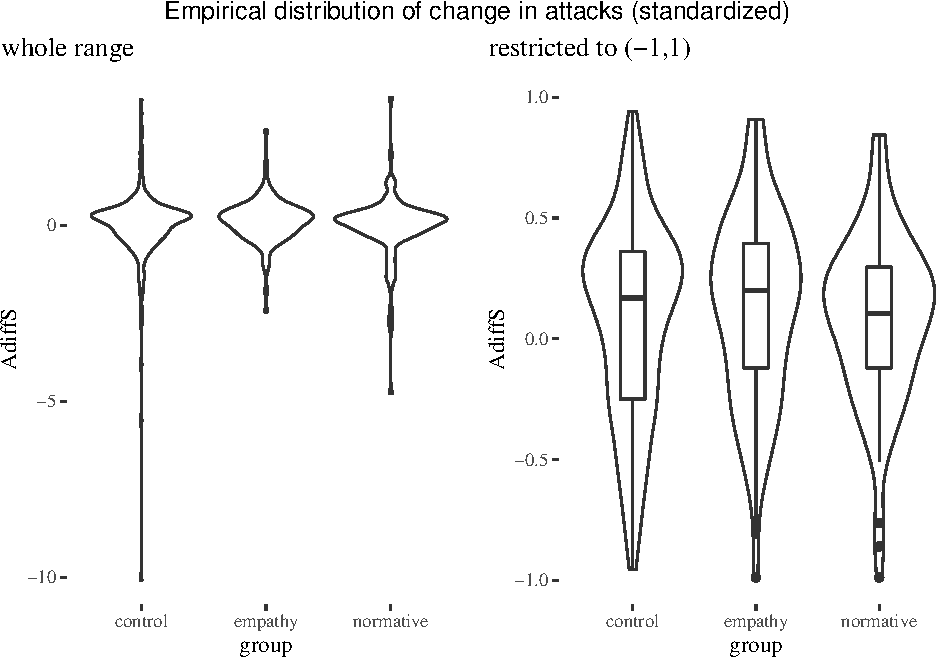
\includegraphics[width=1\linewidth]{technicalReport4_files/figure-latex/violJoint-1} \end{center}
\caption{Empirical distribution of change in attacks, by treatment group.}
\label{fig:violJoint}
\end{figure}

To see how this masking can occur, let's inspect changes in attacks
against intervention counts. It turns out that restricting attention to
various aggression levels in fairly strong changes to the regression
lines (Figure \ref{fig:linearShift}). This suggests we should keep an
eye out for interactions in the analysis, and that the initial
comparison of means or medians between groups might be misleading if the
effects in different volume groups are different and cancel each other.

\vspace{1mm}
\footnotesize

\begin{Shaded}
\begin{Highlighting}[]
\NormalTok{icplot1 }\OtherTok{\textless{}{-}} \FunctionTok{ggplot}\NormalTok{(summaries, }\FunctionTok{aes}\NormalTok{(}\AttributeTok{x =}\NormalTok{ IC, }\AttributeTok{y =}\NormalTok{ AdiffS, }\AttributeTok{color =}\NormalTok{ group, }\AttributeTok{fill =}\NormalTok{ group)) }\SpecialCharTok{+}
    \FunctionTok{geom\_jitter}\NormalTok{(}\AttributeTok{alpha =} \FloatTok{0.6}\NormalTok{, }\AttributeTok{size =} \FloatTok{0.8}\NormalTok{) }\SpecialCharTok{+} \FunctionTok{theme\_tufte}\NormalTok{() }\SpecialCharTok{+} \FunctionTok{theme}\NormalTok{(}\AttributeTok{plot.title.position =} \StringTok{"plot"}\NormalTok{) }\SpecialCharTok{+}
    \FunctionTok{geom\_smooth}\NormalTok{(}\AttributeTok{alpha =} \FloatTok{0.2}\NormalTok{, }\AttributeTok{method =} \StringTok{"lm"}\NormalTok{) }\SpecialCharTok{+} \FunctionTok{xlim}\NormalTok{(}\FunctionTok{c}\NormalTok{(}\DecValTok{0}\NormalTok{, }\DecValTok{25}\NormalTok{)) }\SpecialCharTok{+} \FunctionTok{ylim}\NormalTok{(}\FunctionTok{c}\NormalTok{(}\SpecialCharTok{{-}}\DecValTok{2}\NormalTok{,}
    \DecValTok{2}\NormalTok{)) }\SpecialCharTok{+} \FunctionTok{ggtitle}\NormalTok{(}\StringTok{"sd restricted to ({-}2,2)"}\NormalTok{) }\SpecialCharTok{+} \FunctionTok{theme}\NormalTok{(}\AttributeTok{legend.position =} \FunctionTok{c}\NormalTok{(}\FloatTok{0.65}\NormalTok{,}
    \FloatTok{0.2}\NormalTok{))}

\NormalTok{icplot2 }\OtherTok{\textless{}{-}} \FunctionTok{ggplot}\NormalTok{(summaries, }\FunctionTok{aes}\NormalTok{(}\AttributeTok{x =}\NormalTok{ IC, }\AttributeTok{y =}\NormalTok{ AdiffS, }\AttributeTok{color =}\NormalTok{ group, }\AttributeTok{fill =}\NormalTok{ group)) }\SpecialCharTok{+}
    \FunctionTok{geom\_jitter}\NormalTok{(}\AttributeTok{alpha =} \FloatTok{0.6}\NormalTok{, }\AttributeTok{size =} \FloatTok{0.8}\NormalTok{) }\SpecialCharTok{+} \FunctionTok{theme\_tufte}\NormalTok{() }\SpecialCharTok{+} \FunctionTok{theme}\NormalTok{(}\AttributeTok{plot.title.position =} \StringTok{"plot"}\NormalTok{) }\SpecialCharTok{+}
    \FunctionTok{geom\_smooth}\NormalTok{(}\AttributeTok{alpha =} \FloatTok{0.2}\NormalTok{, }\AttributeTok{method =} \StringTok{"lm"}\NormalTok{) }\SpecialCharTok{+} \FunctionTok{xlim}\NormalTok{(}\FunctionTok{c}\NormalTok{(}\DecValTok{0}\NormalTok{, }\DecValTok{25}\NormalTok{)) }\SpecialCharTok{+} \FunctionTok{ylim}\NormalTok{(}\FunctionTok{c}\NormalTok{(}\SpecialCharTok{{-}}\DecValTok{1}\NormalTok{,}
    \DecValTok{1}\NormalTok{)) }\SpecialCharTok{+} \FunctionTok{ggtitle}\NormalTok{(}\StringTok{"sd restricted to ({-}1,1)"}\NormalTok{) }\SpecialCharTok{+} \FunctionTok{theme}\NormalTok{(}\AttributeTok{legend.position =} \FunctionTok{c}\NormalTok{(}\FloatTok{0.65}\NormalTok{,}
    \FloatTok{0.2}\NormalTok{))}


\NormalTok{icplotJoint }\OtherTok{\textless{}{-}} \FunctionTok{ggarrange}\NormalTok{(icplot1, icplot2)}
\NormalTok{icplotTitled }\OtherTok{\textless{}{-}} \FunctionTok{annotate\_figure}\NormalTok{(icplotJoint, }\AttributeTok{top =} \FunctionTok{text\_grob}\NormalTok{(}\StringTok{"Change in attacks (standardized) vs interventions received"}\NormalTok{,}
    \AttributeTok{size =} \DecValTok{12}\NormalTok{))}
\end{Highlighting}
\end{Shaded}

\normalsize

\begin{figure}

\begin{center}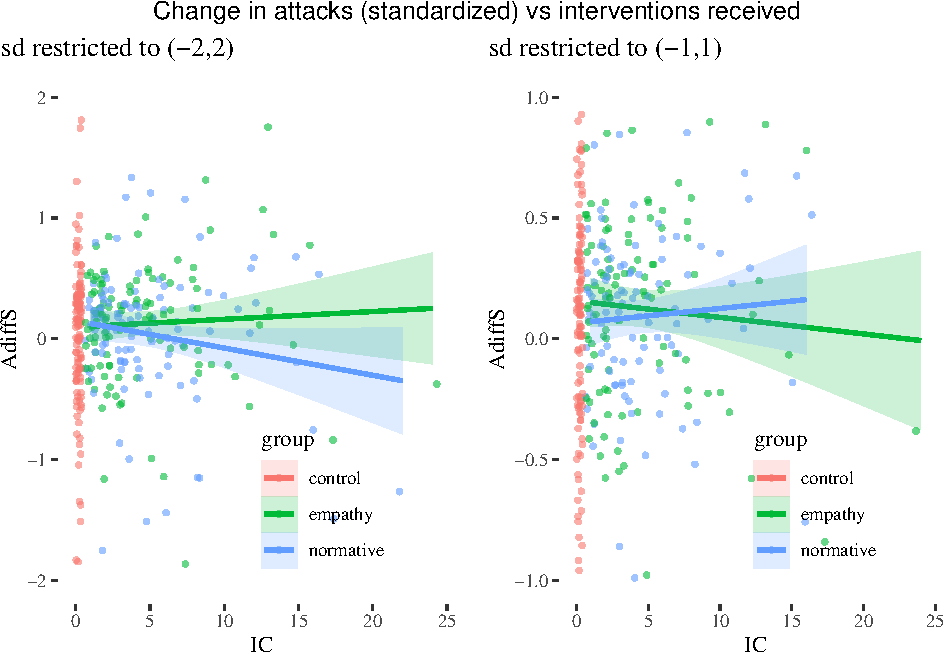
\includegraphics[width=1\linewidth]{technicalReport4_files/figure-latex/fig:linearShift-1} \end{center}
\caption{Change in attacks vs intervention counts by treatment group, jittered with  linear smoothing. Change of range of aggression levels results in different linear smoothings.}
\label{fig:linearShift}
\end{figure}

Let's now inspect correlations between the variables involved in the
model (Figure \ref{fig:correlations}). Almost no predictors are strongly
correlated, except for \textsf{CBS}, \textsf{CAS} and \textsf{CDS}. We
are not interested in using \textsf{CAS} as a predictor, as it occurs
\emph{after} the interventions, and we drop \textsf{CDS} from the
analysis, generally avoiding using these variables in the same model to
avoid statistical issues resulting from multicolinearity. In fact, it is
no surprise that users' general activity in a period is a decent proxy
for their general activity in other periods.

\begin{figure}[H]

\begin{center}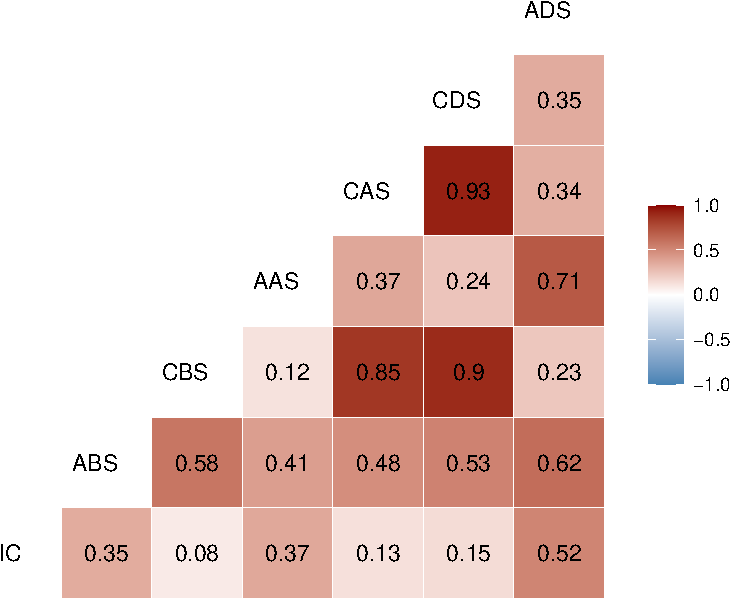
\includegraphics[width=1\linewidth]{technicalReport4_files/figure-latex/correlations-1} \end{center}
\caption{Correlations between predictors used in the before-and-after analysis.}
\label{fig:correlations}
\end{figure}

\hypertarget{causal-inference-and-variable-selection}{%
\section{Causal inference and variable
selection}\label{causal-inference-and-variable-selection}}

To identify the right variables to condition (or not condition) on to
identify the causal effect of the interventions, we first need to think
about the causal structure of the problem. A plausible causal structure
that we will be working with is visualized in Figure \ref{fig:causal}.
Comments during impact attacks during, which trigger interventions.
Unmeasured user features cause comments before, which impact attacks
before, and also attacks before directly. Comments during (their impact
on ADS is already included) impact attacks during during directly and
comments after, which impact attacks after and attacks after directly.
Intervention count impacts attacks after and comments after. The same
directions of impact are included for intervention type. Finally,
comments through time are connected causally, and so are attacks.

\vspace{1mm}
\footnotesize

\begin{Shaded}
\begin{Highlighting}[]
\NormalTok{dag }\OtherTok{\textless{}{-}} \FunctionTok{dagitty}\NormalTok{(}\StringTok{"}
\StringTok{  dag\{}
\StringTok{  CDS {-}\textgreater{} ADS {-}\textgreater{} IC  }
\StringTok{               U [unobserved]   }
\StringTok{               U {-}\textgreater{} CBS {-}\textgreater{} ABS  }
\StringTok{               U {-}\textgreater{} ABS        }
\StringTok{               U {-}\textgreater{} CDS {-}\textgreater{} ADS  }
\StringTok{               U {-}\textgreater{} ADS         }
\StringTok{               U {-}\textgreater{} CAS {-}\textgreater{} AAS    }
\StringTok{               U {-}\textgreater{} AAS                        }
\StringTok{               IC {-}\textgreater{} AAS        }
\StringTok{               IC {-}\textgreater{} CAS        }
\StringTok{               IT {-}\textgreater{} CAS        }
\StringTok{               IT {-}\textgreater{} AAS}
\StringTok{               CBS {-}\textgreater{} CDS {-}\textgreater{} CAS}
\StringTok{               ABS {-}\textgreater{} ADS {-}\textgreater{} AAS}
\StringTok{               \}"}\NormalTok{)}
\FunctionTok{coordinates}\NormalTok{(dag) }\OtherTok{\textless{}{-}} \FunctionTok{list}\NormalTok{(}\AttributeTok{x =} \FunctionTok{c}\NormalTok{(}\AttributeTok{CBS =} \DecValTok{0}\NormalTok{, }\AttributeTok{ABS =} \DecValTok{0}\NormalTok{, }\AttributeTok{CDS =} \DecValTok{1}\NormalTok{, }\AttributeTok{ADS =} \DecValTok{1}\NormalTok{, }\AttributeTok{CAS =} \DecValTok{2}\NormalTok{,}
    \AttributeTok{AAS =} \DecValTok{2}\NormalTok{, }\AttributeTok{IT =} \FloatTok{1.5}\NormalTok{, }\AttributeTok{IC =} \FloatTok{1.5}\NormalTok{, }\AttributeTok{U =} \FloatTok{0.5}\NormalTok{), }\AttributeTok{y =} \FunctionTok{c}\NormalTok{(}\AttributeTok{CBS =} \DecValTok{0}\NormalTok{, }\AttributeTok{ABS =} \DecValTok{1}\NormalTok{, }\AttributeTok{CDS =} \DecValTok{0}\NormalTok{,}
    \AttributeTok{ADS =} \DecValTok{1}\NormalTok{, }\AttributeTok{CAS =} \DecValTok{0}\NormalTok{, }\AttributeTok{AAS =} \DecValTok{1}\NormalTok{, }\AttributeTok{IT =} \FloatTok{0.3}\NormalTok{, }\AttributeTok{IC =} \FloatTok{0.7}\NormalTok{, }\AttributeTok{U =} \FloatTok{0.5}\NormalTok{))}
\end{Highlighting}
\end{Shaded}

\normalsize

\begin{figure}[H]

\begin{center}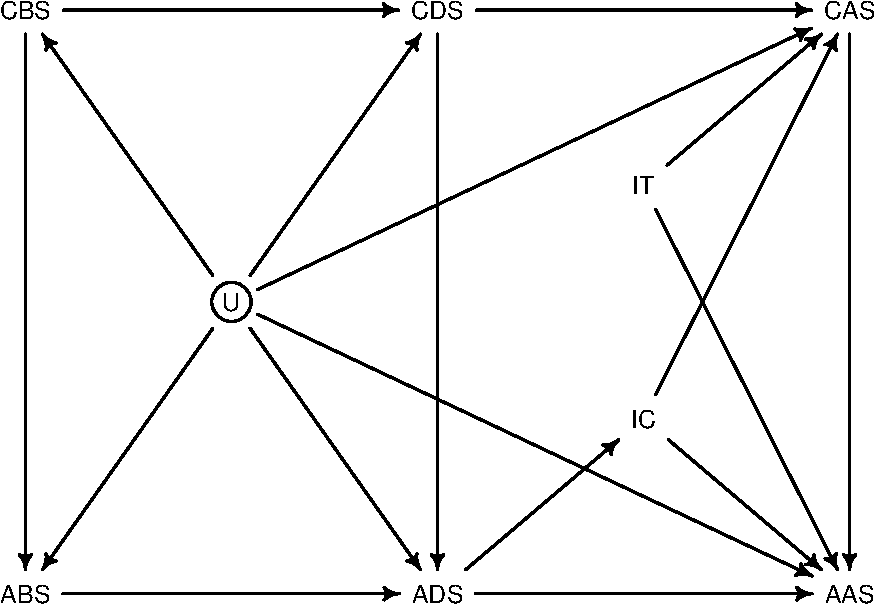
\includegraphics[width=1\linewidth]{technicalReport4_files/figure-latex/unnamed-chunk-5-1} \end{center}
\caption{A causal model used in the before-and-after analysis.}
\label{fig:causal}
\end{figure}

We already know not to condition on CDS if we condition on CAS or CBS
(multicolinearity). What else can we learn from the causal model?
\textsf{IT} has no backdoor paths, but \textsf{IC} does, so we need to
make sure these are closed to avoid including spurious correlations in
our analysis. There are in fact 65 different paths from \textsf{IC} to
\textsf{AAC}. Crucially, all backdoor paths go through \textsf{ADS},
which then becomes either a fork or a pipe, so all backdoor paths can be
closed by conditioning on \textsf{ADS}. Moreover there is only one
directed indirect path, it goes through \textsf{CAS}, so we should not
condition on \textsf{CAS} if we are to identify total causal effect of
\textsf{IC} on attacks, including the impact mediated by its impact on
comments (unless we care about the direct effect of \textsf{IC} and
\textsf{IT} on \textsf{AAS}, but that's a separate question). This is in
line with the adjustment set identified algorithmically using by the
\textsf{dagitty} package.

The situation is somewhat different when it comes to evaluating the
\emph{direct} effect of intervention. Then, we also need to block
indirect causal paths from the intervention to the outcome. For such an
evaluation we need to also condition on \textsf{CAS}, which is what we
will do when we turn to the study of the direct effects of the
interventions.

\vspace{1mm}
\footnotesize

\begin{Shaded}
\begin{Highlighting}[]
\FunctionTok{paths}\NormalTok{(dag, }\AttributeTok{from =} \FunctionTok{c}\NormalTok{(}\StringTok{"IC"}\NormalTok{), }\AttributeTok{to =} \StringTok{"AAS"}\NormalTok{)}
\end{Highlighting}
\end{Shaded}

\begin{verbatim}
## $paths
##  [1] "IC -> AAS"                                              
##  [2] "IC -> CAS -> AAS"                                       
##  [3] "IC -> CAS <- CDS -> ADS -> AAS"                         
##  [4] "IC -> CAS <- CDS -> ADS <- ABS <- CBS <- U -> AAS"      
##  [5] "IC -> CAS <- CDS -> ADS <- ABS <- U -> AAS"             
##  [6] "IC -> CAS <- CDS -> ADS <- U -> AAS"                    
##  [7] "IC -> CAS <- CDS <- CBS -> ABS -> ADS -> AAS"           
##  [8] "IC -> CAS <- CDS <- CBS -> ABS -> ADS <- U -> AAS"      
##  [9] "IC -> CAS <- CDS <- CBS -> ABS <- U -> AAS"             
## [10] "IC -> CAS <- CDS <- CBS -> ABS <- U -> ADS -> AAS"      
## [11] "IC -> CAS <- CDS <- CBS <- U -> AAS"                    
## [12] "IC -> CAS <- CDS <- CBS <- U -> ABS -> ADS -> AAS"      
## [13] "IC -> CAS <- CDS <- CBS <- U -> ADS -> AAS"             
## [14] "IC -> CAS <- CDS <- U -> AAS"                           
## [15] "IC -> CAS <- CDS <- U -> ABS -> ADS -> AAS"             
## [16] "IC -> CAS <- CDS <- U -> ADS -> AAS"                    
## [17] "IC -> CAS <- CDS <- U -> CBS -> ABS -> ADS -> AAS"      
## [18] "IC -> CAS <- IT -> AAS"                                 
## [19] "IC -> CAS <- U -> AAS"                                  
## [20] "IC -> CAS <- U -> ABS -> ADS -> AAS"                    
## [21] "IC -> CAS <- U -> ABS <- CBS -> CDS -> ADS -> AAS"      
## [22] "IC -> CAS <- U -> ADS -> AAS"                           
## [23] "IC -> CAS <- U -> CBS -> ABS -> ADS -> AAS"             
## [24] "IC -> CAS <- U -> CBS -> CDS -> ADS -> AAS"             
## [25] "IC -> CAS <- U -> CDS -> ADS -> AAS"                    
## [26] "IC -> CAS <- U -> CDS <- CBS -> ABS -> ADS -> AAS"      
## [27] "IC <- ADS -> AAS"                                       
## [28] "IC <- ADS <- ABS <- CBS -> CDS -> CAS -> AAS"           
## [29] "IC <- ADS <- ABS <- CBS -> CDS -> CAS <- IT -> AAS"     
## [30] "IC <- ADS <- ABS <- CBS -> CDS -> CAS <- U -> AAS"      
## [31] "IC <- ADS <- ABS <- CBS -> CDS <- U -> AAS"             
## [32] "IC <- ADS <- ABS <- CBS -> CDS <- U -> CAS -> AAS"      
## [33] "IC <- ADS <- ABS <- CBS -> CDS <- U -> CAS <- IT -> AAS"
## [34] "IC <- ADS <- ABS <- CBS <- U -> AAS"                    
## [35] "IC <- ADS <- ABS <- CBS <- U -> CAS -> AAS"             
## [36] "IC <- ADS <- ABS <- CBS <- U -> CAS <- IT -> AAS"       
## [37] "IC <- ADS <- ABS <- CBS <- U -> CDS -> CAS -> AAS"      
## [38] "IC <- ADS <- ABS <- CBS <- U -> CDS -> CAS <- IT -> AAS"
## [39] "IC <- ADS <- ABS <- U -> AAS"                           
## [40] "IC <- ADS <- ABS <- U -> CAS -> AAS"                    
## [41] "IC <- ADS <- ABS <- U -> CAS <- IT -> AAS"              
## [42] "IC <- ADS <- ABS <- U -> CBS -> CDS -> CAS -> AAS"      
## [43] "IC <- ADS <- ABS <- U -> CBS -> CDS -> CAS <- IT -> AAS"
## [44] "IC <- ADS <- ABS <- U -> CDS -> CAS -> AAS"             
## [45] "IC <- ADS <- ABS <- U -> CDS -> CAS <- IT -> AAS"       
## [46] "IC <- ADS <- CDS -> CAS -> AAS"                         
## [47] "IC <- ADS <- CDS -> CAS <- IT -> AAS"                   
## [48] "IC <- ADS <- CDS -> CAS <- U -> AAS"                    
## [49] "IC <- ADS <- CDS <- CBS -> ABS <- U -> AAS"             
## [50] "IC <- ADS <- CDS <- CBS -> ABS <- U -> CAS -> AAS"      
## [51] "IC <- ADS <- CDS <- CBS -> ABS <- U -> CAS <- IT -> AAS"
## [52] "IC <- ADS <- CDS <- CBS <- U -> AAS"                    
## [53] "IC <- ADS <- CDS <- CBS <- U -> CAS -> AAS"             
## [54] "IC <- ADS <- CDS <- CBS <- U -> CAS <- IT -> AAS"       
## [55] "IC <- ADS <- CDS <- U -> AAS"                           
## [56] "IC <- ADS <- CDS <- U -> CAS -> AAS"                    
## [57] "IC <- ADS <- CDS <- U -> CAS <- IT -> AAS"              
## [58] "IC <- ADS <- U -> AAS"                                  
## [59] "IC <- ADS <- U -> ABS <- CBS -> CDS -> CAS -> AAS"      
## [60] "IC <- ADS <- U -> ABS <- CBS -> CDS -> CAS <- IT -> AAS"
## [61] "IC <- ADS <- U -> CAS -> AAS"                           
## [62] "IC <- ADS <- U -> CAS <- IT -> AAS"                     
## [63] "IC <- ADS <- U -> CBS -> CDS -> CAS -> AAS"             
## [64] "IC <- ADS <- U -> CBS -> CDS -> CAS <- IT -> AAS"       
## [65] "IC <- ADS <- U -> CDS -> CAS -> AAS"                    
## [66] "IC <- ADS <- U -> CDS -> CAS <- IT -> AAS"              
## 
## $open
##  [1]  TRUE  TRUE FALSE FALSE FALSE FALSE FALSE FALSE FALSE FALSE FALSE FALSE
## [13] FALSE FALSE FALSE FALSE FALSE FALSE FALSE FALSE FALSE FALSE FALSE FALSE
## [25] FALSE FALSE  TRUE  TRUE FALSE FALSE FALSE FALSE FALSE  TRUE  TRUE FALSE
## [37]  TRUE FALSE  TRUE  TRUE FALSE  TRUE FALSE  TRUE FALSE  TRUE FALSE FALSE
## [49] FALSE FALSE FALSE  TRUE  TRUE FALSE  TRUE  TRUE FALSE  TRUE FALSE FALSE
## [61]  TRUE FALSE  TRUE FALSE  TRUE FALSE
\end{verbatim}

\begin{Shaded}
\begin{Highlighting}[]
\FunctionTok{adjustmentSets}\NormalTok{(dag, }\AttributeTok{exposure =} \FunctionTok{c}\NormalTok{(}\StringTok{"IC"}\NormalTok{, }\StringTok{"IT"}\NormalTok{), }\AttributeTok{outcome =} \StringTok{"AAS"}\NormalTok{, }\AttributeTok{type =} \StringTok{"all"}\NormalTok{)}
\end{Highlighting}
\end{Shaded}

\begin{verbatim}
## { ADS }
## { ABS, ADS }
## { ADS, CBS }
## { ABS, ADS, CBS }
## { ADS, CDS }
## { ABS, ADS, CDS }
## { ADS, CBS, CDS }
## { ABS, ADS, CBS, CDS }
## { ADS, U }
## { ABS, ADS, U }
## { ADS, CBS, U }
## { ABS, ADS, CBS, U }
## { ADS, CDS, U }
## { ABS, ADS, CDS, U }
## { ADS, CBS, CDS, U }
## { ABS, ADS, CBS, CDS, U }
\end{verbatim}

\normalsize

In fact, we will be predicting the difference between attacks before and
after, and the difference between comments, before and after, but the
general points about the nodes involved apply also to defined nodes.
Finding a maximal sensible set (canonical) of covariates suggests
including \textsf{CDS} and \textsf{ABS}. As already discussed, we do not
include \textsf{CDS} because of its strong correlation with
\textsf{CBS}. We also do not condition on \textsf{ABS}---not only
because it has a pretty strong correlation with another predictor
(\textsf{ADS}), but rather mainly because it is used to define the
output variable. In such a set-up, it is clear that a model including
\textsf{ABS} would have better predictive power, but since a
definitional connection is present, thinking that its inclusion in the
model tells us something about causality would be misled.

Otherwise, it's open season for the other variables and interactions
between them, and our decision to include or exclude them in the model
will be guided by information-theoretic criteria of predictive power.

\hypertarget{before-and-after-analysis-bayesian-model-building}{%
\section{Before-and-after analysis: bayesian model
building}\label{before-and-after-analysis-bayesian-model-building}}

We build and compared multiple additive models where the outcome
variable is normally distributed around the predicted mean, which is a
linear function of predictors (possibly with interactions). Bayesian
information criteria (WAIC)\footnote{
Here's a more detailed explanation of the model comparison method we used, uninterested reader is invited to skip forward. Let  $y$ be the observations and $\Theta$  a posterior distribution.
First, log-pointwise-predictive-density is defined by:
\begin{align*}
\mathsf{lppd}(y, \Theta) & = \sum_i log\frac{1}{S}\sum_s p (y_i\vert \Theta_s)
\end{align*}
\noindent where $S$ is the number of samples in the posterior, and $\Theta_s$ 
is the $s$-th combination of sampled parameter values in the posterior distribution. That is, 
for each observation and each combination of 
parameters in the posterior we first compute its density, then 
we take the average density of that observation over all combinations of parameters in the posterior,
and  then take the logarithm. Finally, we sum these values up for all the observations. Crucially, when comparing posterior distributions with respect to the same dataset, \textsf{lppd}s are proportional
 to unbiased estimates of their divergence from the real distribution (note that it is \emph{only} 
 proportional, and for this reason can be used for comparison of distributions 
 only and makes no intuitive sense on its own).  However, \textsf{lppd} always improves
  as the model gets more complex, so for model comparison it makes more sense to use 
 the Widely Applicable Information Criterion (WAIC), which is an approximation of the out-of-sample deviance that converges to the cross-validation approximation in a large sample. It  is defined as
 the log-posterior-predictive-density with an additional
  penalty proportional to the variance in the
  posterior predictions:
  \begin{align*}
\mathsf{WAIC(y, \Theta)} & = -2 (\mathsf{lppd} - \overbrace{\sum_i var_\theta \mathsf{log} p (y_i \vert \theta)}^{\mathsf{penalty}})
  \end{align*}
\noindent  Thus to construct the penalty, we calculate the variance in log-probabilities for each observation and sum them up. Because of the analogy to Akaike's criterion, the penalty is sometimes called the effective number of parameters, $p_{\mathsf{WAIC}}$. 
How does WAIC compare to other information criteria?  AIC uses MAP estimates instead of the posterior and requires that priors be flat or overwhelmed by the likelihood, and assumes that the posterior distribution is approximately multivariate Gaussian and the sample size is  much greater  than the number of parameters used in the model. Bayesian Information Criterion (BIC) also requires flat priors and uses MAP estimates. WAIC does not make these assumptions, and provides almost exactly the same results as AIC, when AIC’s assumptions are met.}
applied to a wide selection of predictors lead to the model, whose
specification is as follows (we also selected regularizing prior
parameters using prior predictive checks to avoid unreasonably narrow
overall prior distributions):

\vspace{-2mm}

\begin{align*}
\mathsf{AdiffS} & \sim \textsf{Norm}(\mu, \sigma)\\
\mu_i & = \alpha + \beta_{\mathsf{ADS}}[\mathsf{group}_i]\times \mathsf{ADS} + \beta_{\mathsf{group}_i}  +
 \beta_{\mathsf{IC}}[\mathsf{group}_i]\times \mathsf{IC} + \\
 & + \beta_{\mathsf{ADSIC}}\times \mathsf{ADS} \times \mathsf{IC} + \beta_{\mathsf{CBS}}[\mathsf{group}_i] \times \mathsf{CBS}\\
 \alpha & \sim \textsf{Norm}(0,.3)\\
\beta_{\mathsf{ADS}}[\mathsf{group}_i] & \sim \textsf{Norm}(0,.3)\\
\beta_{\mathsf{group}_i} & \sim \textsf{Norm}(0,.3)\\
\beta_{\mathsf{IC}}[\mathsf{group}_i] & \sim \textsf{Norm}(0,.3)\\
 \beta_{\mathsf{ADSIC}} & \sim \textsf{Norm}(0,.3)\\
 \beta_{\mathsf{CBS}}[\mathsf{group}_i]& \sim \textsf{Norm}(0,.3)\\
\end{align*}

That is, we take the resulting mean to be the result of the general
average (\(\alpha\)) and the impact of the following coefficients:
group-specific coefficient for \textsf{ADS}, group coefficient,
group-specific coefficient for \textsf{IC}, interaction coefficient for
\textsf{ADS} and \textsf{IC}, and group-specific coefficient for
\textsf{CBS}. This is plausible \emph{prima facie} which group a user
belongs to might have impact on how attacks during the treatment is
related to attacks after, the role of the intervention count, and the
role of comments before. Moreover, the levels of aggressive behavior
displayed by the user during treatment might have impact on the role
played by the intervention count.

\vspace{1mm}
\footnotesize

\begin{Shaded}
\begin{Highlighting}[]
\CommentTok{\# building model with sd=1}
\NormalTok{InteractionsModelDiffSD1 }\OtherTok{\textless{}{-}} \FunctionTok{ulam}\NormalTok{(}
  \FunctionTok{alist}\NormalTok{(}
\NormalTok{    AdiffS }\SpecialCharTok{\textasciitilde{}} \FunctionTok{dnorm}\NormalTok{( mu, sigma ),}
\NormalTok{    mu }\OtherTok{\textless{}{-}}\NormalTok{ a }\SpecialCharTok{+}\NormalTok{ bADS[groupID] }\SpecialCharTok{*}\NormalTok{ ADS }\SpecialCharTok{+}\NormalTok{  bIT[groupID] }\SpecialCharTok{+}\NormalTok{ bIC[groupID] }\SpecialCharTok{*}\NormalTok{ IC}\SpecialCharTok{+}
\NormalTok{    bADSIC }\SpecialCharTok{*}\NormalTok{ ADS }\SpecialCharTok{*}\NormalTok{ IC}\SpecialCharTok{+}\NormalTok{ bCBS[groupID] }\SpecialCharTok{*}\NormalTok{CBS,}
\NormalTok{    a }\SpecialCharTok{\textasciitilde{}} \FunctionTok{dnorm}\NormalTok{ (}\DecValTok{0}\NormalTok{,}\DecValTok{1}\NormalTok{),}
\NormalTok{    bADS[groupID] }\SpecialCharTok{\textasciitilde{}} \FunctionTok{dnorm}\NormalTok{(}\DecValTok{0}\NormalTok{,}\DecValTok{1}\NormalTok{),}
\NormalTok{    bADSIC }\SpecialCharTok{\textasciitilde{}} \FunctionTok{dnorm}\NormalTok{(}\DecValTok{0}\NormalTok{,}\DecValTok{1}\NormalTok{),}
\NormalTok{    bCBS[groupID] }\SpecialCharTok{\textasciitilde{}} \FunctionTok{dnorm}\NormalTok{(}\DecValTok{0}\NormalTok{,}\DecValTok{1}\NormalTok{),}
\NormalTok{    bIT[groupID] }\SpecialCharTok{\textasciitilde{}} \FunctionTok{dnorm}\NormalTok{(}\DecValTok{0}\NormalTok{,}\DecValTok{1}\NormalTok{),}
\NormalTok{    bIC[groupID] }\SpecialCharTok{\textasciitilde{}} \FunctionTok{dnorm}\NormalTok{(}\DecValTok{0}\NormalTok{,}\DecValTok{1}\NormalTok{),}
\NormalTok{    sigma  }\SpecialCharTok{\textasciitilde{}} \FunctionTok{dexp}\NormalTok{(}\DecValTok{1}\NormalTok{)}
\NormalTok{  ),}
  \AttributeTok{data =}\NormalTok{ summaries}
\NormalTok{ )}
 
\CommentTok{\#saveRDS(InteractionsModelDiffSD1, file = "models/InteractionsModelDiffSD1.rds")}
\NormalTok{InteractionsModelDiffSD1 }\OtherTok{\textless{}{-}} \FunctionTok{readRDS}\NormalTok{(}\AttributeTok{file =} \StringTok{"models/InteractionsModelDiffSD1.rds"}\NormalTok{)}


\CommentTok{\#now model with prior sd = .3}
\NormalTok{InteractionsModelDiff }\OtherTok{\textless{}{-}} \FunctionTok{ulam}\NormalTok{(}
  \FunctionTok{alist}\NormalTok{(}
\NormalTok{    AdiffS }\SpecialCharTok{\textasciitilde{}} \FunctionTok{dnorm}\NormalTok{( mu, sigma ),}
\NormalTok{    mu }\OtherTok{\textless{}{-}}\NormalTok{ a }\SpecialCharTok{+}\NormalTok{ bADS[groupID] }\SpecialCharTok{*}\NormalTok{ ADS }\SpecialCharTok{+}\NormalTok{  bIT[groupID] }\SpecialCharTok{+}\NormalTok{ bIC[groupID] }\SpecialCharTok{*}\NormalTok{ IC }\SpecialCharTok{+}
\NormalTok{    bADSIC }\SpecialCharTok{*}\NormalTok{ ADS }\SpecialCharTok{*}\NormalTok{ IC}\SpecialCharTok{+}\NormalTok{ bCBS[groupID] }\SpecialCharTok{*}\NormalTok{CBS,}
\NormalTok{    a }\SpecialCharTok{\textasciitilde{}} \FunctionTok{dnorm}\NormalTok{ (}\DecValTok{0}\NormalTok{,}\FloatTok{0.3}\NormalTok{),}
\NormalTok{    bADS[groupID] }\SpecialCharTok{\textasciitilde{}} \FunctionTok{dnorm}\NormalTok{(}\DecValTok{0}\NormalTok{,.}\DecValTok{3}\NormalTok{),}
\NormalTok{    bADSIC }\SpecialCharTok{\textasciitilde{}} \FunctionTok{dnorm}\NormalTok{(}\DecValTok{0}\NormalTok{,.}\DecValTok{3}\NormalTok{),}
\NormalTok{    bCBS[groupID] }\SpecialCharTok{\textasciitilde{}} \FunctionTok{dnorm}\NormalTok{(}\DecValTok{0}\NormalTok{,.}\DecValTok{3}\NormalTok{),}
\NormalTok{    bIT[groupID] }\SpecialCharTok{\textasciitilde{}} \FunctionTok{dnorm}\NormalTok{(}\DecValTok{0}\NormalTok{,.}\DecValTok{3}\NormalTok{),}
\NormalTok{    bIC[groupID] }\SpecialCharTok{\textasciitilde{}} \FunctionTok{dnorm}\NormalTok{(}\DecValTok{0}\NormalTok{,.}\DecValTok{3}\NormalTok{),}
\NormalTok{    sigma  }\SpecialCharTok{\textasciitilde{}} \FunctionTok{dexp}\NormalTok{(}\DecValTok{1}\NormalTok{)}
\NormalTok{  ),}
  \AttributeTok{data =}\NormalTok{ summaries}
\NormalTok{)}

\CommentTok{\#saveRDS(InteractionsModelDiff, file = "models/InteractionsModelDiff.rds")}

\NormalTok{InteractionsModelDiff }\OtherTok{\textless{}{-}} \FunctionTok{readRDS}\NormalTok{(}\AttributeTok{file =} \StringTok{"models/InteractionsModelDiff.rds"}\NormalTok{)}

\CommentTok{\#prior predictive checks sd =1}
\NormalTok{ADS }\OtherTok{\textless{}{-}} \DecValTok{0}
\NormalTok{CBS }\OtherTok{\textless{}{-}} \DecValTok{0}
\NormalTok{groupID }\OtherTok{\textless{}{-}} \DecValTok{1}\SpecialCharTok{:}\DecValTok{3}
\NormalTok{IC }\OtherTok{\textless{}{-}} \DecValTok{5}  \CommentTok{\#mean for interventions in treatment}
\NormalTok{data }\OtherTok{\textless{}{-}} \FunctionTok{expand.grid}\NormalTok{(}\AttributeTok{ADS =}\NormalTok{ ADS,}\AttributeTok{groupID =}\NormalTok{ groupID, }\AttributeTok{CBS =}\NormalTok{ CBS, }\AttributeTok{IC =}\NormalTok{  IC)}
\NormalTok{prior }\OtherTok{\textless{}{-}} \FunctionTok{extract.prior}\NormalTok{(InteractionsModelDiffSD1, }\AttributeTok{n =} \FloatTok{1e4}\NormalTok{)}
\NormalTok{mu }\OtherTok{\textless{}{-}} \FunctionTok{link}\NormalTok{( InteractionsModelDiffSD1 , }\AttributeTok{post=}\NormalTok{prior , }\AttributeTok{data=}\NormalTok{data )}
\FunctionTok{colnames}\NormalTok{(mu) }\OtherTok{\textless{}{-}} \FunctionTok{levels}\NormalTok{(summaries}\SpecialCharTok{$}\NormalTok{group)}
\NormalTok{muLong }\OtherTok{\textless{}{-}} \FunctionTok{melt}\NormalTok{(mu)}
\FunctionTok{colnames}\NormalTok{(muLong) }\OtherTok{\textless{}{-}} \FunctionTok{c}\NormalTok{(}\StringTok{"id"}\NormalTok{, }\StringTok{"group"}\NormalTok{, }\StringTok{"AdiffS"}\NormalTok{)}

\NormalTok{priorGroupsSD1 }\OtherTok{\textless{}{-}} \FunctionTok{ggplot}\NormalTok{(muLong)}\SpecialCharTok{+}
  \FunctionTok{geom\_violin}\NormalTok{(}\FunctionTok{aes}\NormalTok{(}\AttributeTok{x =}\NormalTok{ group, }\AttributeTok{y =}\NormalTok{ AdiffS))}\SpecialCharTok{+}
  \FunctionTok{theme\_tufte}\NormalTok{()}\SpecialCharTok{+}\FunctionTok{xlab}\NormalTok{(}\StringTok{""}\NormalTok{)}\SpecialCharTok{+}
  \FunctionTok{labs}\NormalTok{(}\AttributeTok{title =} \StringTok{"Simulated priors by group"}\NormalTok{,}
  \AttributeTok{subtitle =} \StringTok{"(at ADS = CBS = 0, IC at mean = 5, sd = 1)"}\NormalTok{)}\SpecialCharTok{+}
  \FunctionTok{ylab}\NormalTok{(}\StringTok{"change in attacks (standardized)"}\NormalTok{)}

\NormalTok{ADS }\OtherTok{\textless{}{-}} \DecValTok{0}
\NormalTok{CBS }\OtherTok{\textless{}{-}} \DecValTok{0}
\NormalTok{groupID }\OtherTok{\textless{}{-}} \DecValTok{1}\SpecialCharTok{:}\DecValTok{3}
\NormalTok{IC }\OtherTok{\textless{}{-}} \DecValTok{0}\SpecialCharTok{:}\DecValTok{20}
\NormalTok{data }\OtherTok{\textless{}{-}} \FunctionTok{expand.grid}\NormalTok{(}\AttributeTok{ADS =}\NormalTok{ ADS,}\AttributeTok{groupID =}\NormalTok{ groupID, }\AttributeTok{CBS =}\NormalTok{ CBS, }\AttributeTok{IC =}\NormalTok{  IC)}

\NormalTok{prior }\OtherTok{\textless{}{-}} \FunctionTok{extract.prior}\NormalTok{(InteractionsModelDiffSD1, }\AttributeTok{n =} \FloatTok{1e4}\NormalTok{)}
\NormalTok{mu }\OtherTok{\textless{}{-}} \FunctionTok{link}\NormalTok{(InteractionsModelDiffSD1 , }\AttributeTok{post=}\NormalTok{prior , }\AttributeTok{data=}\NormalTok{data )}
\NormalTok{mu.mean }\OtherTok{\textless{}{-}} \FunctionTok{apply}\NormalTok{( mu , }\DecValTok{2}\NormalTok{, mean )}
\NormalTok{mu.HPDI }\OtherTok{\textless{}{-}} \FunctionTok{data.frame}\NormalTok{(}\FunctionTok{t}\NormalTok{(}\FunctionTok{apply}\NormalTok{( mu , }\DecValTok{2}\NormalTok{ , HPDI )))}
\NormalTok{priorDF }\OtherTok{\textless{}{-}} \FunctionTok{cbind}\NormalTok{(data, mu.mean, mu.HPDI)}
\NormalTok{priorDF}\SpecialCharTok{$}\NormalTok{groupID }\OtherTok{\textless{}{-}} \FunctionTok{as.factor}\NormalTok{(groupID)}
\FunctionTok{levels}\NormalTok{(priorDF}\SpecialCharTok{$}\NormalTok{groupID) }\OtherTok{\textless{}{-}} \FunctionTok{c}\NormalTok{(}\StringTok{"control"}\NormalTok{, }\StringTok{"empathy"}\NormalTok{, }\StringTok{"normative"}\NormalTok{)}
\FunctionTok{colnames}\NormalTok{(priorDF)[}\DecValTok{2}\NormalTok{]}\OtherTok{\textless{}{-}} \StringTok{"group"}


\NormalTok{priorICSD1  }\OtherTok{\textless{}{-}} \FunctionTok{ggplot}\NormalTok{(priorDF, }\FunctionTok{aes}\NormalTok{(}\AttributeTok{x =}\NormalTok{ IC, }\AttributeTok{y  =}\NormalTok{ mu.mean,  }\AttributeTok{fill =}\NormalTok{ group))}\SpecialCharTok{+}
  \FunctionTok{geom\_line}\NormalTok{()}\SpecialCharTok{+}\FunctionTok{geom\_ribbon}\NormalTok{(}\FunctionTok{aes}\NormalTok{(}\AttributeTok{ymin =}\NormalTok{ X.}\FloatTok{0.89}\NormalTok{, }\AttributeTok{ymax =}\NormalTok{ X0.}\FloatTok{89.}\NormalTok{), }\AttributeTok{alpha =} \FloatTok{0.2}\NormalTok{)}\SpecialCharTok{+}
  \FunctionTok{theme\_tufte}\NormalTok{()}\SpecialCharTok{+}\FunctionTok{ylab}\NormalTok{(}\StringTok{"change in attacks (standardized)"}\NormalTok{)}\SpecialCharTok{+}
  \FunctionTok{labs}\NormalTok{(}\AttributeTok{title =} \StringTok{"Simulated priors for AAS vs IC"}\NormalTok{,}
      \AttributeTok{subtitle =} \StringTok{"(at ADS = CBS = 0, sd = 1)"}\NormalTok{)}\SpecialCharTok{+}\FunctionTok{xlab}\NormalTok{(}\StringTok{"interventions"}\NormalTok{)}


\NormalTok{priorJoint1 }\OtherTok{\textless{}{-}} \FunctionTok{ggarrange}\NormalTok{(priorGroupsSD1,priorICSD1, }\AttributeTok{ncol =} \DecValTok{2}\NormalTok{)}
\NormalTok{priorJoint1Titled }\OtherTok{\textless{}{-}} \FunctionTok{annotate\_figure}\NormalTok{(priorJoint1,}
  \AttributeTok{top =} \FunctionTok{text\_grob}\NormalTok{(}\StringTok{"Predictive priors with sd=1 are insanely wide"}\NormalTok{,}
                  \AttributeTok{size =} \DecValTok{14}\NormalTok{))}
\NormalTok{priorJoint1Titled}

\CommentTok{\#Some experimentation leads to the value of $\textbackslash{}sigma =.3$, which leads to the following priors:}

\NormalTok{prior predictive check sd }\OtherTok{=}\NormalTok{.}\DecValTok{3}
\NormalTok{ADS }\OtherTok{\textless{}{-}} \DecValTok{0}
\NormalTok{CBS }\OtherTok{\textless{}{-}} \DecValTok{0}
\NormalTok{groupID }\OtherTok{\textless{}{-}} \DecValTok{1}\SpecialCharTok{:}\DecValTok{3}
\NormalTok{IC }\OtherTok{\textless{}{-}} \DecValTok{5}  \CommentTok{\#mean for interventions in treatment}
\NormalTok{data }\OtherTok{\textless{}{-}} \FunctionTok{expand.grid}\NormalTok{(}\AttributeTok{ADS =}\NormalTok{ ADS,}\AttributeTok{groupID =}\NormalTok{ groupID, }\AttributeTok{CBS =}\NormalTok{ CBS, }\AttributeTok{IC =}\NormalTok{  IC)}
\NormalTok{prior }\OtherTok{\textless{}{-}} \FunctionTok{extract.prior}\NormalTok{(InteractionsModelDiff, }\AttributeTok{n =} \FloatTok{1e4}\NormalTok{)}
\NormalTok{mu }\OtherTok{\textless{}{-}} \FunctionTok{link}\NormalTok{(InteractionsModelDiff , }\AttributeTok{post=}\NormalTok{prior , }\AttributeTok{data=}\NormalTok{data ) }
\FunctionTok{colnames}\NormalTok{(mu) }\OtherTok{\textless{}{-}} \FunctionTok{levels}\NormalTok{(summaries}\SpecialCharTok{$}\NormalTok{group)}
\NormalTok{muLong }\OtherTok{\textless{}{-}} \FunctionTok{melt}\NormalTok{(mu)}
\FunctionTok{colnames}\NormalTok{(muLong) }\OtherTok{\textless{}{-}} \FunctionTok{c}\NormalTok{(}\StringTok{"id"}\NormalTok{, }\StringTok{"group"}\NormalTok{, }\StringTok{"AdiffS"}\NormalTok{)}
\FunctionTok{head}\NormalTok{(muLong)}

\NormalTok{priorGroupSD03 }\OtherTok{\textless{}{-}} \FunctionTok{ggplot}\NormalTok{(muLong)}\SpecialCharTok{+}
  \FunctionTok{geom\_violin}\NormalTok{(}\FunctionTok{aes}\NormalTok{(}\AttributeTok{x =}\NormalTok{ group, }\AttributeTok{y =}\NormalTok{ AdiffS))}\SpecialCharTok{+}\FunctionTok{theme\_tufte}\NormalTok{()}\SpecialCharTok{+}
  \FunctionTok{xlab}\NormalTok{(}\StringTok{""}\NormalTok{)}\SpecialCharTok{+}
  \FunctionTok{labs}\NormalTok{(}\AttributeTok{title =} \StringTok{"Simulated priors  by group"}\NormalTok{, }
  \AttributeTok{subtitle =} \StringTok{"(at ADS = CBS = 0, IC at mean = 5, sd = .3)"}\NormalTok{)}\SpecialCharTok{+}
  \FunctionTok{ylab}\NormalTok{(}\StringTok{"change in attacks (standarized)"}\NormalTok{)}

\NormalTok{ADS }\OtherTok{\textless{}{-}} \DecValTok{0}
\NormalTok{CBS }\OtherTok{\textless{}{-}} \DecValTok{0}
\NormalTok{groupID }\OtherTok{\textless{}{-}} \DecValTok{1}\SpecialCharTok{:}\DecValTok{3}
\NormalTok{IC }\OtherTok{\textless{}{-}} \DecValTok{5}  \CommentTok{\#mean for interventions in treatment}
\NormalTok{data }\OtherTok{\textless{}{-}} \FunctionTok{expand.grid}\NormalTok{(}\AttributeTok{ADS =}\NormalTok{ ADS,}\AttributeTok{groupID =}\NormalTok{ groupID, }\AttributeTok{CBS =}\NormalTok{ CBS, }\AttributeTok{IC =}\NormalTok{  IC)}
\NormalTok{prior }\OtherTok{\textless{}{-}} \FunctionTok{extract.prior}\NormalTok{(InteractionsModelDiffSD1, }\AttributeTok{n =} \FloatTok{1e4}\NormalTok{)}
\NormalTok{mu }\OtherTok{\textless{}{-}} \FunctionTok{link}\NormalTok{( InteractionsModelDiffSD1 , }\AttributeTok{post=}\NormalTok{prior , }\AttributeTok{data=}\NormalTok{data ) }
\FunctionTok{colnames}\NormalTok{(mu) }\OtherTok{\textless{}{-}} \FunctionTok{levels}\NormalTok{(summaries}\SpecialCharTok{$}\NormalTok{group)}
\NormalTok{muLong }\OtherTok{\textless{}{-}} \FunctionTok{melt}\NormalTok{(mu)}
\FunctionTok{colnames}\NormalTok{(muLong) }\OtherTok{\textless{}{-}} \FunctionTok{c}\NormalTok{(}\StringTok{"id"}\NormalTok{, }\StringTok{"group"}\NormalTok{, }\StringTok{"AdiffS"}\NormalTok{)}
\FunctionTok{head}\NormalTok{(muLong)}

\NormalTok{priorICSD03 }\OtherTok{\textless{}{-}} \FunctionTok{ggplot}\NormalTok{(muLong)}\SpecialCharTok{+}
  \FunctionTok{geom\_violin}\NormalTok{(}\FunctionTok{aes}\NormalTok{(}\AttributeTok{x =}\NormalTok{ group, }\AttributeTok{y =}\NormalTok{ AdiffS))}\SpecialCharTok{+}
  \FunctionTok{theme\_tufte}\NormalTok{()}\SpecialCharTok{+}\FunctionTok{xlab}\NormalTok{(}\StringTok{""}\NormalTok{)}\SpecialCharTok{+}
  \FunctionTok{labs}\NormalTok{(}\AttributeTok{title =} \StringTok{"Simulated priors by group"}\NormalTok{, }
  \AttributeTok{subtitle =} \StringTok{"(at ADS = CBS = 0, IC at mean = 5, sd = 1)"}\NormalTok{)}\SpecialCharTok{+}
  \FunctionTok{ylab}\NormalTok{(}\StringTok{"change in attacks (standardized)"}\NormalTok{)}

\NormalTok{priorJoint03 }\OtherTok{\textless{}{-}} \FunctionTok{ggarrange}\NormalTok{(priorGroupSD03,priorICSD03, }\AttributeTok{ncol =} \DecValTok{2}\NormalTok{) }
\NormalTok{priorJoint03Titled }\OtherTok{\textless{}{-}} \FunctionTok{annotate\_figure}\NormalTok{(priorJoint03, }
  \AttributeTok{top =} \FunctionTok{text\_grob}\NormalTok{(}\StringTok{"Predictive priors with sd=.3 seem sensible"}\NormalTok{,}
                  \AttributeTok{size =} \DecValTok{14}\NormalTok{))}
\NormalTok{priorJoint03Titled}
\end{Highlighting}
\end{Shaded}

\normalsize

Now, some model diagnostics before we move on (Figure
\ref{fig:traceplot}). What we are witnessing is (1) stationarity (the
chains stay mostly in the most probable regions), (2) good mixing (they
explore a range of options in the beginning), and (3) convergence (they
stabilize as they progress). We also need to inspect the distribution of
residuals, expecting them to be more or less normally distributed, which
they are (Figure \ref{fig:residuals}).

\begin{figure}

\begin{center}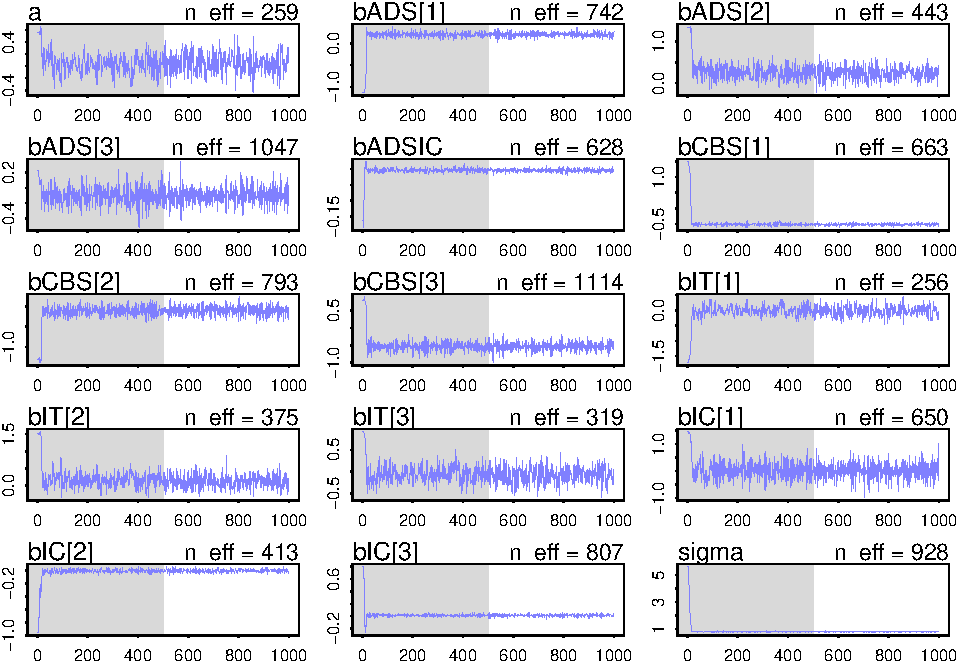
\includegraphics[width=1\linewidth]{technicalReport4_files/figure-latex/traceplot-1} \end{center}
\caption{Traceplot of the model selected using Widelly Acceptable Information Criterion.}
\label{fig:traceplot}
\end{figure}

\vspace{1mm}
\footnotesize

\begin{center}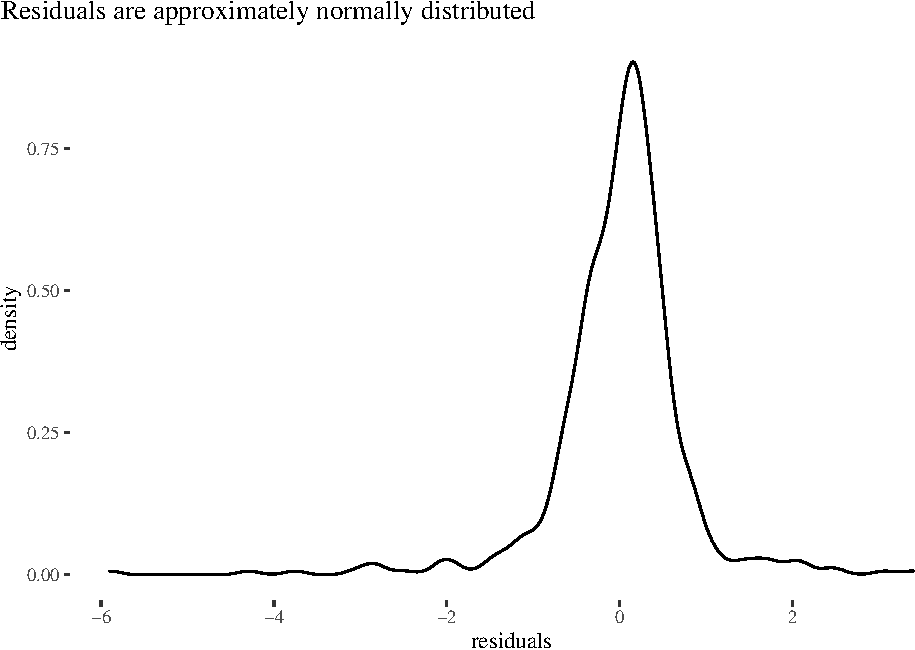
\includegraphics[width=1\linewidth]{technicalReport4_files/figure-latex/unnamed-chunk-8-1} \end{center}
\caption{Distribution of residuals from the selected model.}
\label{fig:residuals}

\textbackslash end\{figure\}

\hypertarget{before-and-after-analysis-results}{%
\section{Before-and-after analysis:
results}\label{before-and-after-analysis-results}}

\end{document}
